\chapter{Introducción}
\label{cap:introduccion}

\chapterquote{We are stubborn on vision. We are flexible on details…}{Jeff Bezos}

\section{Motivación}
Profinder nace del concepto de agilizar y simplificar las relaciones entre profesionales que ofrecen un servicio y usuarios que están dispuestos a consumirlo.

Se trata de una aplicación móvil, inicialmente desarrollada 
para el sistema operativo android (pese a esto no se descarta la posibilidad de poder hacerla multiplataforma en un futuro, véase el capítulo \ref{cap:conclusiones}) en la que tanto usuarios como profesionales se podrán registrar, creando una cuenta e interactuar entre ellos. Las funcionalidades para cada tipo de actor varían en distintos aspectos, manteniendo algunas funcionalidades comunes.  

A continuación se explica la idea de flujo de publicación, contratación y calificación de servicios de la aplicación:
\begin{enumerate}
	\item Al registrarse, los profesionales seleccionaran la categoría de profesional a la que pertenecen -esta categoría podrá ser modificada en cualquier momento desde la pantalla de 'Editar perfil'-.
	\item Una vez registrados, tendrán la posibilidad de crear servicios que a su vez estarán clasificados en categorías y podrán ser públicos o privados (activos o inactivos).
	\item Los servicios activos aparecerán a los usuarios que podrán solicitarlos ya sea desde la pantalla de listado de servicios o a través del perfil del profesional.
	\item Al crear una solicitud un usuario, esta le aparece al profesional que podrá aceptarla o rechazarla. En caso de aceptarla, el trabajo se pone en marcha y en adelante hasta que termine se mostrará como trabajo activo.
	\item Una vez terminado el trabajo, el profesional lo marcará como tal y calificará con estrellas (del 1 al 5) al usuario. Para el profesional el trabajo habrá terminado.
	\item Por último al usuario le aparecerá la opción de calificar al profesional de la misma forma. Una vez hecho esto, el trabajo se marca como completado y se da por terminado el flujo de servicos.
\end{enumerate}
A parte de este flujo en el que cada actor tiene un papel marcado. Hay cierta funcionalidad común, descrita a continuación. Usuarios y profesionales podrán chatear entre sí usando la pantalla de chat, donde podrán concretar fechas y horarios concretos y detalles adicionales. Todos los usuarios y profesionales podrán ser añadidos a listas de favoritos para un fácil acceso a sus perfiles. El perfil de cada actor en la aplicación podrá ser completado con atributos como una descripción o una foto de perfil.

\section{Objetivos}
El mundo del desarrollo android es inmenso, la forma de diseñar interfaces respecto a la programación web muy distinta, y se trata de un mundo que en los últimos años ha estado en constante cambio, cada año salen nuevas tecnologías que dejan obsoleta la que ya había e incluso hace unos años cambió el lenguaje de programación usado para crear aplicaciones android.

El objetivo principal de este trabajo es aprender muchas de las cosas necesarias para ser un desarrollador android competente, partiendo de cero hasta llegar a ser capaz de crear una aplicación robusta, bonita y escalable en el tiempo. 

Los objetivos relativos a la aplicación marcados desde el comienzo se muestran a continuación:
\begin{itemize}
	\item definición de una especificación de requisitos inicial, sujeta a cambios a lo largo del proceso de desarollo, en la que se definen los actores y casos de uso de la aplicación (vease el apéndice \ref{Appendix:srs}).
	\item Una vez definida la especificación de requisitos, se marcarán una serie de hitos para la entrega de las funcionalidades.
\end{itemize}

También se han definido una serie de objetivos técnicos que serán llevados a cabo en paralelo a la consecución de los objetivos relativos a la aplicación:
\begin{itemize}
	\item Aprender kotlin hasta alcanzar un nivel de competencia en el lenguaje apto para el desarrollo.
	\item Empezar en el desarrollo android utilizando el sistema de vistas \footnote{Artículo que hace una introducción al sistema de vistas: \url{https://www.studytonight.com/android/introduction-to-views} }, forma clásica de desarrollar interfaces en android, que sirve como primer acercamiento pese a que luego se sustituya por Jetpack Compose\footnote{\url{https://developer.android.com/develop/ui/compose}}. 
	\item Realizar un acercamiento a las arquitecturas, patrones de diseño y buenas prácticas más utillizadas con el objetivo de empezar a hacer proyectos más robustos que se acerquen a la estructura de proyecto final.
	\item Aprender los fundamentos de Jetpack Compose e ir adquiriendo nuevos conocimientos progresivamente haciendo distintos proyectos de prueba.
	\item Familiarizarse con las distintos servicios de Firebase \footnote{\url{https://firebase.google.com/}} para aplicaciones android que serán usados como backend en la aplicación final.
	\item Al final del proceso de desarrollo de la aplicación se espera haber obtenido una base de conocimientos sólidos que sirvan como punto de partida de una posible carrera profesional futura.
\end{itemize}

\section{Plan de trabajo}
Para la consecución de los objetivos descritos en el apartado anterior, se ha establecido al inicio del proyecto un plan de trabajo representado con un diagrama de Gantt, los objetivos se han dividido -igual que en el apartado anterior- en objetivos técnicos y de aplicación ya que la idea inicial es ir cumpliendo los dos tipos de objetivos en paralelo en el tiempo.
\begin{figure}[h]
	\centering
	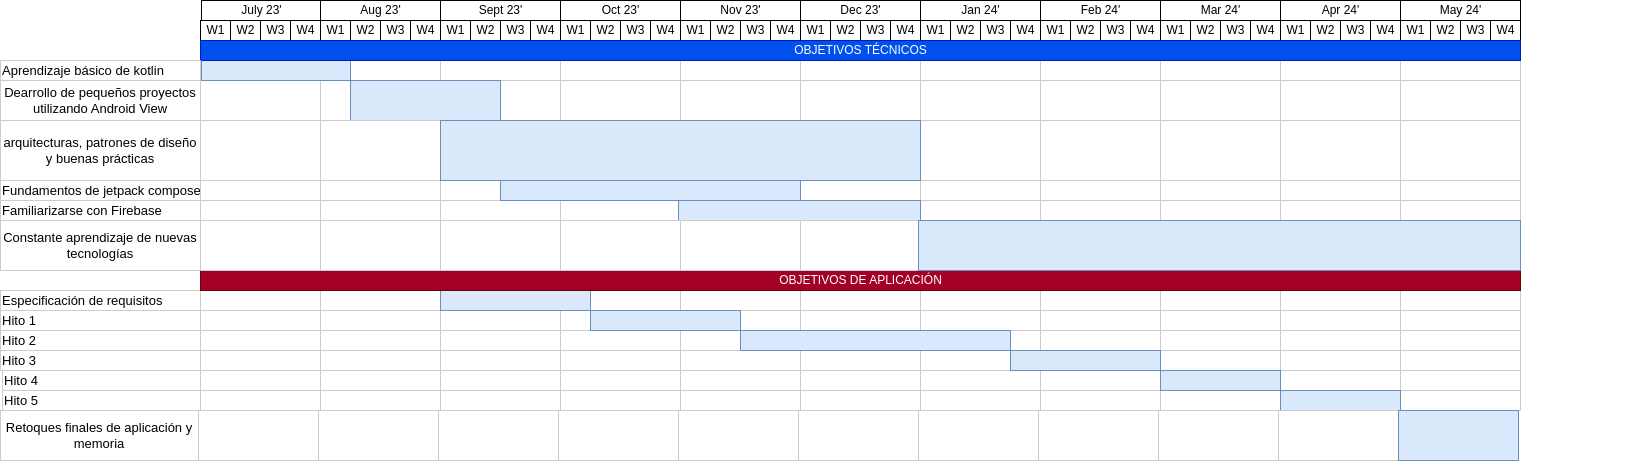
\includegraphics[width = 1\textwidth]{Imagenes/Bitmap/Gantt_Diagram.png}
	\caption{Diagrama de Gantt del proyecto}
	\label{fig:Gantt}
\end{figure}
Respecto a los objetivos hitos del proyecto, a continuación se muestra una lista con los casos de uso a desarrollar en cada hito:
\begin{itemize}
	\item Hito 1
	\begin{itemize}
		\item Registro/baja de usuario.
		\item Modificar datos usuario.
		\item Login/Logout de usuario.
		\item Configurar app.
	\end{itemize}
	\item Hito 2
	\begin{itemize}
		\item Cambiar estado de profesional.
		\item Dar de alta/baja servicio.
		\item Modificar servicio.
		\item Listar servicios dados de alta.
		\item Añadir/eliminar/Modificar categorías de servicios ofrecidos.
	\end{itemize}
	\item Hito 3
	\begin{itemize}
		\item Buscar servicio.
		\item Configurar búsqueda.
		\item Consultar profesional.
		\item Consultar cliente.
		\item Añadir/Quitar Profesional de lista de favoritos.
		\item Añadir/Modificar/Quitar cliente de lista de favoritos.
		\item Ver lista de favoritos.
	\end{itemize}
	\item Hito 4
	\begin{itemize}
		\item Contratar servicio.
		\item Chatear con profesional/cliente.
		\item Valorar cliente/profesional.
		\item Contestar solicitud de contratación.
	\end{itemize}
	\item Hito 5
	\begin{itemize}
		\item Consultar datos/estadísticas de profesional/clientes.
		\item Buscar clientes/profesionales.
		\item Modificar datos de clientes/profesionales/servicios ofrecidos.
		\item Dar de baja usuarios.
	\end{itemize}
\end{itemize}
Debido a que los casos de uso eran una aproximación inicial, según ha ido avanzando el proceso de desarrollo, algunos casos de uso se han implementado antes, después, o se han descartado por no encajar bien en la aplicación. A pesar de esto, la planificación inicial ha sido de gran utilidad como guía y ha servido para marcar correctamente los plazos de entrega, asimilando el proceso a como sería en un entorno real.